
\documentclass[11pt,a4paper]{article}
\usepackage[T1]{fontenc}
\usepackage[utf8]{inputenc}
\usepackage{lmodern}
\usepackage[margin=24mm]{geometry}
\usepackage{graphicx}
\usepackage{amsmath,amssymb}
\usepackage{booktabs}
\usepackage{array}
\usepackage{float}
\usepackage{caption}
\usepackage{xurl}
\usepackage{hyperref}
\usepackage[numbers,sort&compress]{natbib}
\usepackage{setspace}
\hypersetup{colorlinks=true,linkcolor=black,citecolor=black,urlcolor=blue}
\setstretch{1.10}

\title{Dynamical Threshold Theory of Sleep:\\
A Claim-Bounded Integrated Model and Audit Synthesis for Sleep-Like Recovery Transitions\\
\large v0.3.1 Integrated Revision}
\author{Keiji Yoshimura\\\small Independent Researcher}
\date{May 25, 2026}

\begin{document}
\maketitle

\begin{center}
\small
Repository: \url{https://github.com/yokken0907/dynamical-threshold-theory-of-sleep}\\
License: source-defined Evaluation-Only Notice in the repository.
\end{center}

\begin{abstract}
This integrated revision combines the original Dynamical Threshold Theory of Sleep (DTTS) model manuscript with the subsequent v0.2.0--v0.2.8 audit sequence and v0.3.0 synthesis addendum. DTTS is treated here as a claim-bounded network-dynamical prototype for sleep-like recovery transitions in finite adaptive networks. The original model represents a multicellular system as a graph of adaptively coupled oscillatory elements carrying local homeostatic load, local sleep propensity, and selectively protected interactions. Wake-like dynamics are represented as noisy adaptive synchronization under continued perturbation, while sleep-like dynamics emerge when local load accumulation and coherence degradation drive a thresholded recovery gate into a sleep-dominant renormalization regime. The audit sequence adds threshold, hysteresis, perturbation-recovery, topology/noise, failure-boundary, rescue-classification, and frozen holdout tests. Across the tested toy-model envelope, threshold-like gate onset, hysteresis-like persistence, structurally aligned selective protection, and rescue-sensitive regimes were observed. However, expanded audits also identified failure boundaries, and weak-protection conditions remained unstable under harsher holdout. This manuscript does not claim clinical sleep modeling, biological sleep validation, EEG or wearable-device prediction, diagnosis, treatment guidance, or a complete theory of physiological sleep.
\end{abstract}

\paragraph{Reader guidance and medical non-claim.}
This manuscript is a mathematical and computational prototype study. It is not medical advice, not a clinical sleep model, not a diagnostic or treatment tool, and not a claim of validation against human or animal sleep data. All results should be interpreted as reduced network-dynamical evidence for sleep-like recovery-transition behavior inside the implemented toy-model and audit settings.

\section{Introduction}
Sleep is associated with homeostatic recovery, local use-dependent regulation, state-dependent reorganization of network interactions, and temporally structured circadian gating. Major explanatory traditions emphasize synaptic homeostasis and down-selection \cite{Tononi2003,Tononi2006,Cirelli2015,Tononi2014}, local sleep-like events and use-dependent regional regulation \cite{Vyazovskiy2011,Krueger2019,Siclari2018}, and two-process homeostatic/circadian regulation \cite{Borbely2022,Deboer2018}. These traditions are individually productive, but they are often expressed at different levels of description.

DTTS was proposed to express these motifs in a single reduced dynamical language. The aim is not to replace biological sleep science with a toy model. The aim is narrower: to ask whether a finite adaptive network with local load, local coherence, a thresholded sleep-like gate, and protected coupling updates can produce recovery-transition motifs that are mathematically closed and numerically auditable.

Synchronization models, including the Kuramoto family and small-world network synchronization studies, provide a natural mathematical background for treating collective coherence and its degradation \cite{Acebron2005,Hong2002}. DTTS extends that reduced language by adding local burden variables, sleep-like gate dynamics, and selective coupling renormalization.

\section{Model}
\subsection{Network and phase dynamics}
We represent the system as a network of $N$ coupled oscillatory nodes on an undirected graph $G=(V,E)$ with adjacency matrix $A_{ij}\in\{0,1\}$. Each node has phase $\theta_i(t)$, intrinsic frequency $\omega_i$, local sleep gate $q_i(t)$, and perturbation susceptibility $\sigma_i$. The phase dynamics are
\begin{equation}
\frac{d\theta_i}{dt}=\omega_i+\sum_{j=1}^{N}A_{ij}K_{ij}\sin(\theta_j-\theta_i)+\sigma_i(1-q_i)\xi_i(t),
\end{equation}
where $K_{ij}$ is the adaptive coupling and $\xi_i(t)$ denotes independent Gaussian noise. Local coherence is
\begin{equation}
R_i(t)=\left|\frac{1}{d_i}\sum_{j=1}^{N}A_{ij}e^{i(\theta_j-\theta_i)}\right|.
\end{equation}

\subsection{Local load and sleep-like gate}
Each node carries homeostatic load $s_i(t)$:
\begin{equation}
\frac{ds_i}{dt}=a(1-R_i)+\chi u_i(t)-bq_i s_i,
\end{equation}
where $u_i(t)$ is a localized use-dependent drive. The sleep-like gate evolves according to
\begin{equation}
\tau_q\frac{dq_i}{dt}=-q_i+\Sigma\left(\beta_s(s_i-s_c)-\beta_c C(t)-\beta_R(R_i-R_c)\right),
\end{equation}
where $C(t)$ is a circadian-like permissive term and $\Sigma$ is a sigmoid. In this reduced setting, ``sleep-like'' means only a modeled recovery-gate transition. It does not mean physiological sleep.

\subsection{Selective protection and coupling updates}
Adaptive coupling weights are updated by
\begin{equation}
\frac{dK_{ij}}{dt}=(1-\bar q_{ij})\left[\eta_W P_{ij}(K_{\max}-K_{ij})-\delta_W K_{ij}\right]-\bar q_{ij}\eta_K(\mu K_{ij}-\kappa P_{ij}),
\end{equation}
where $P_{ij}$ is a protection field representing prior structural/coherence history. During a sleep-dominant interval, couplings relax toward the protection-dependent fixed point
\begin{equation}
K^*_{ij}=\frac{\kappa}{\mu}P_{ij}.
\end{equation}

\section{Reduced free-energy closure}
A key purpose of the original DTTS formulation was to avoid unbounded adaptive-coupling pathologies. In the sleep-dominant limit, the dynamics can be written as a gradient flow of a reduced free energy
\begin{equation}
\mathcal{F}_s(K,s\mid P)=\sum_{i<j}A_{ij}\left(\frac{\mu}{2}K_{ij}^2-\kappa P_{ij}K_{ij}\right)+\frac{\nu}{2}\sum_i s_i^2.
\end{equation}
In the limit $q_i\to1$, the coupling and load dynamics satisfy $\dot K_{ij}\propto-\partial\mathcal{F}_s/\partial K_{ij}$ and $\dot s_i\propto-\partial\mathcal{F}_s/\partial s_i$, giving $d\mathcal{F}_s/dt\le0$ within the reduced subsystem.

\section{Original proof-of-concept diagnostics}
The original DTTS numerical prototype used a hierarchical modular small-world network with localized filtered-Poisson drive. Figure~\ref{fig:timeseries} summarizes the core behavior: local burden accumulates, mean sleep propensity rises into a sleep-dominant regime, mean coupling strength downscales toward a finite band, and the reduced free energy relaxes after an initial transient.

\begin{figure}[H]
\centering
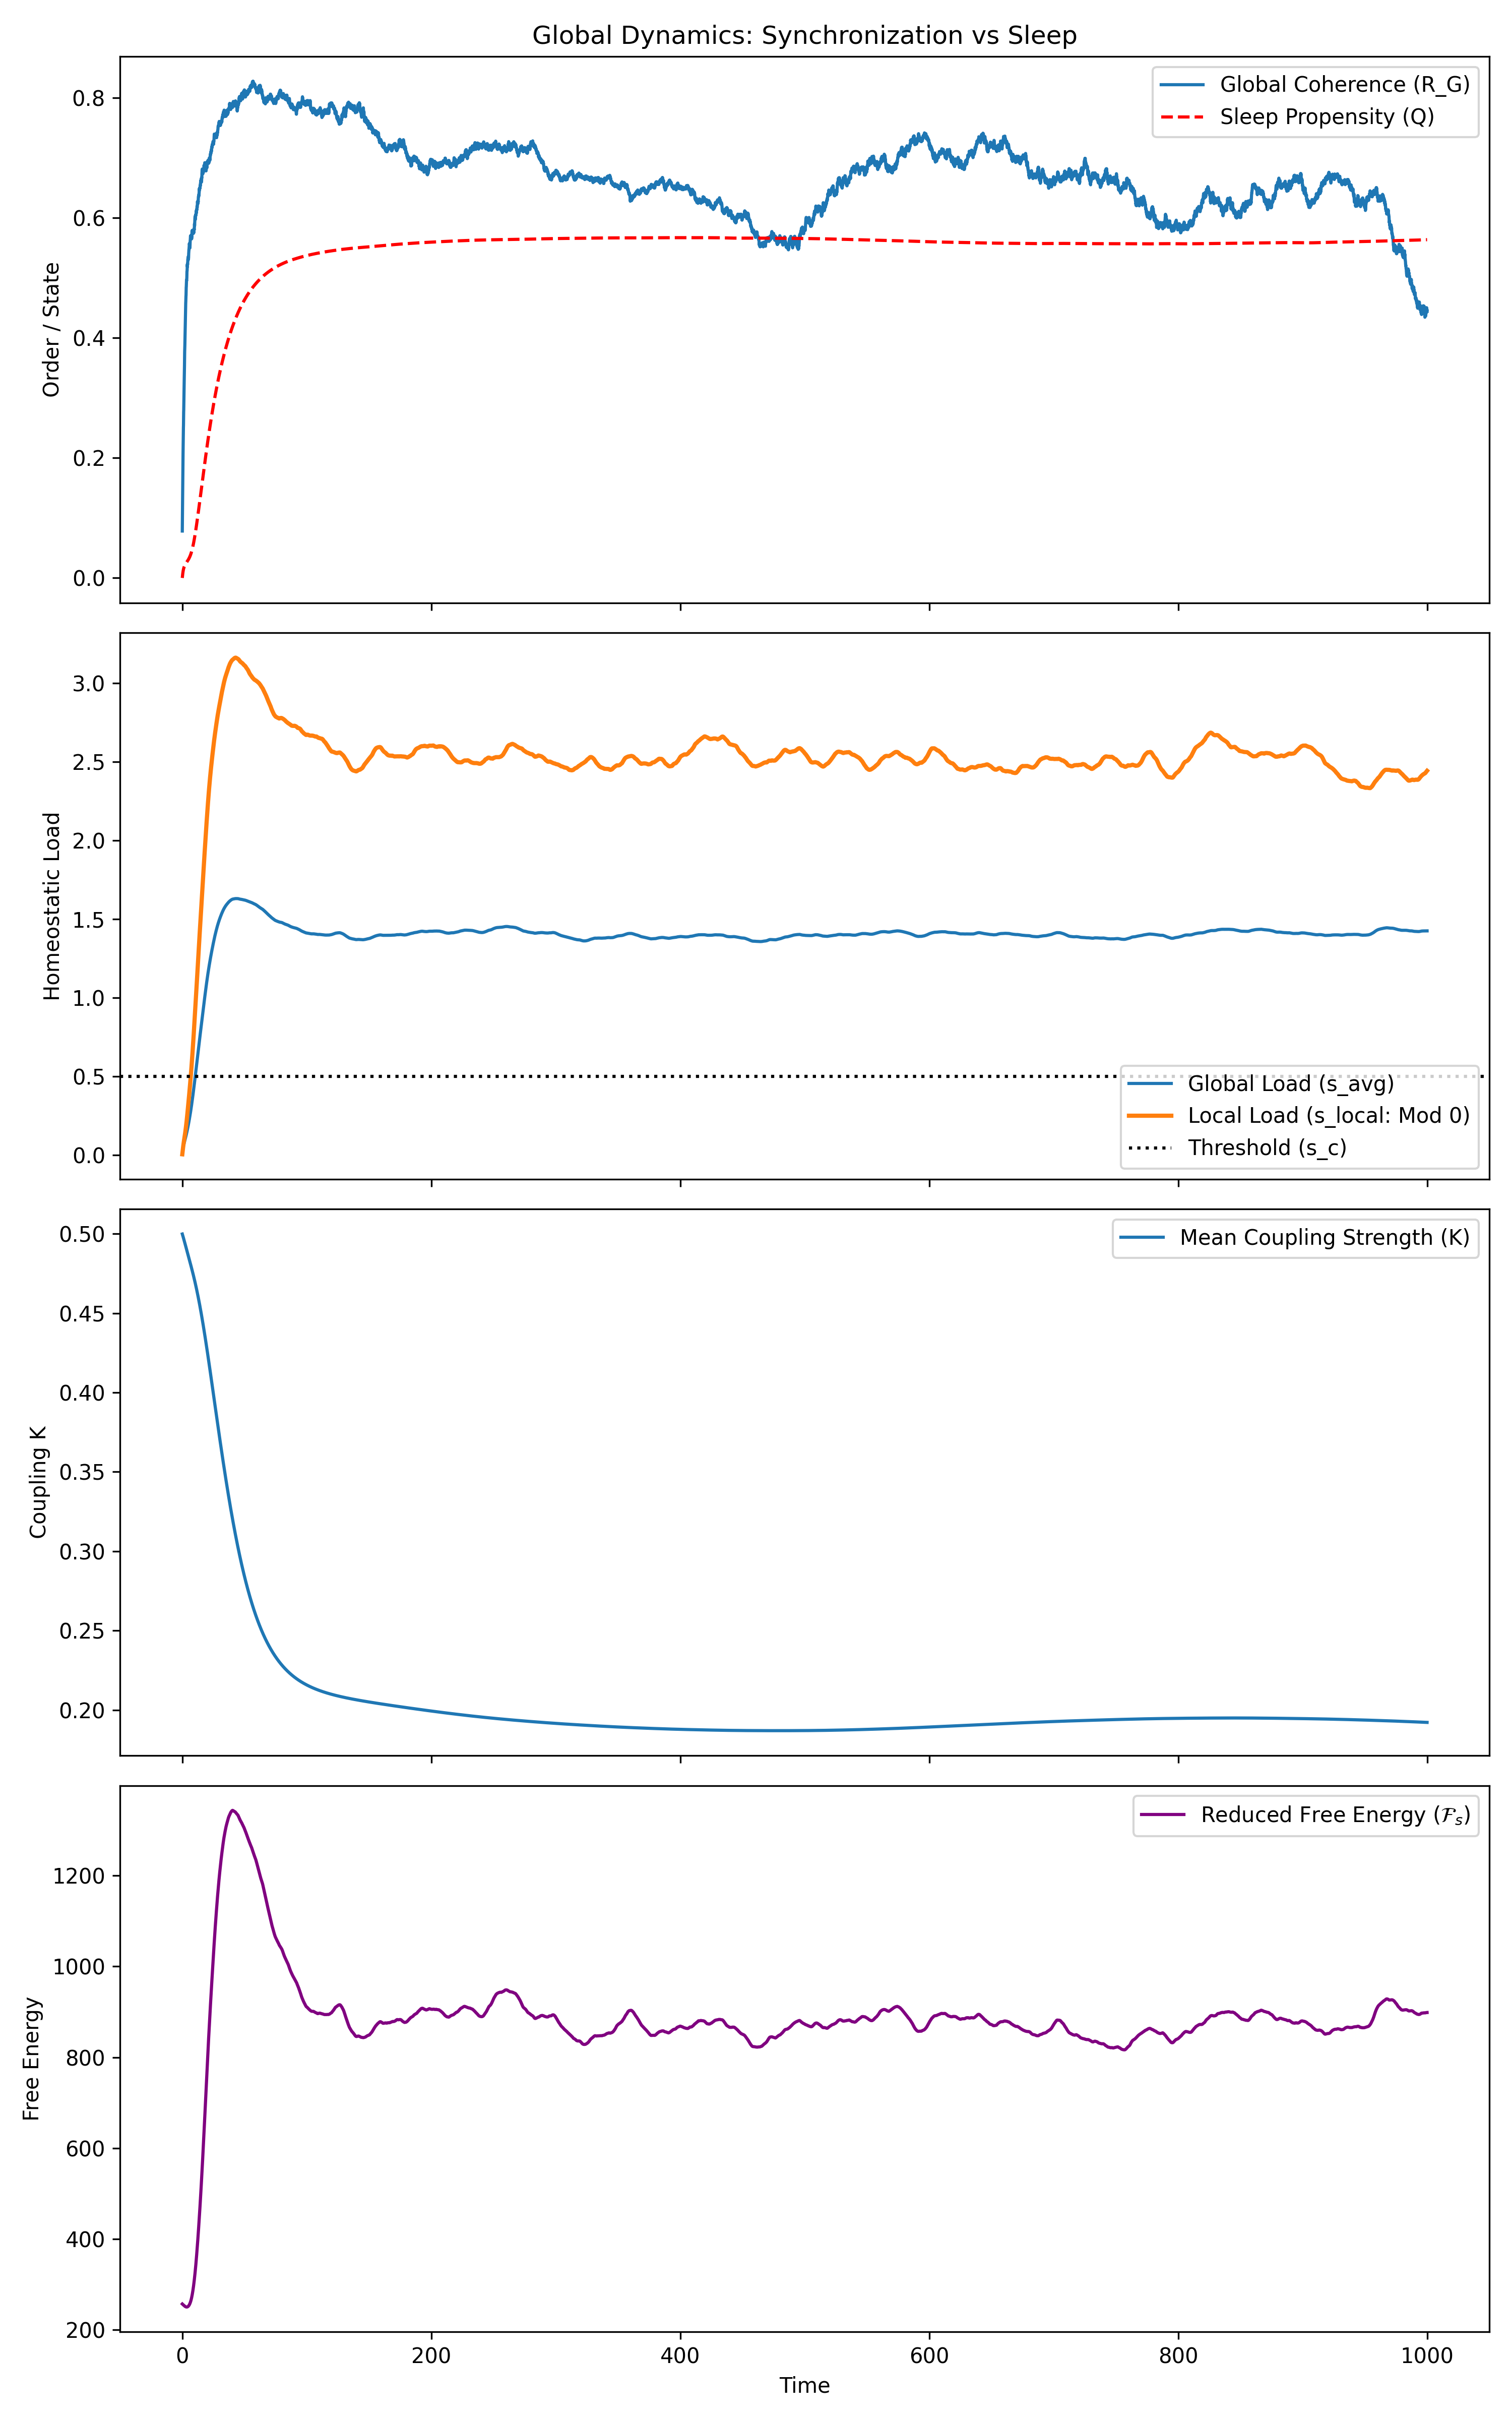
\includegraphics[width=0.78\linewidth]{fig_timeseries_final.png}
\caption{Original DTTS simulation summary. Top to bottom: global coherence $R_G$ and mean sleep propensity $Q$; homeostatic load; mean coupling strength; and reduced free energy. This is a proof-of-concept network-dynamical diagnostic, not a biological sleep-data fit.}
\label{fig:timeseries}
\end{figure}

The original selective-protection diagnostic is shown in Figure~\ref{fig:scatter}. Edges with higher pre-sleep protection were relatively preserved, while less protected edges were more strongly down-selected. This supports the model-internal idea of selective renormalization rather than uniform weakening.

\begin{figure}[H]
\centering
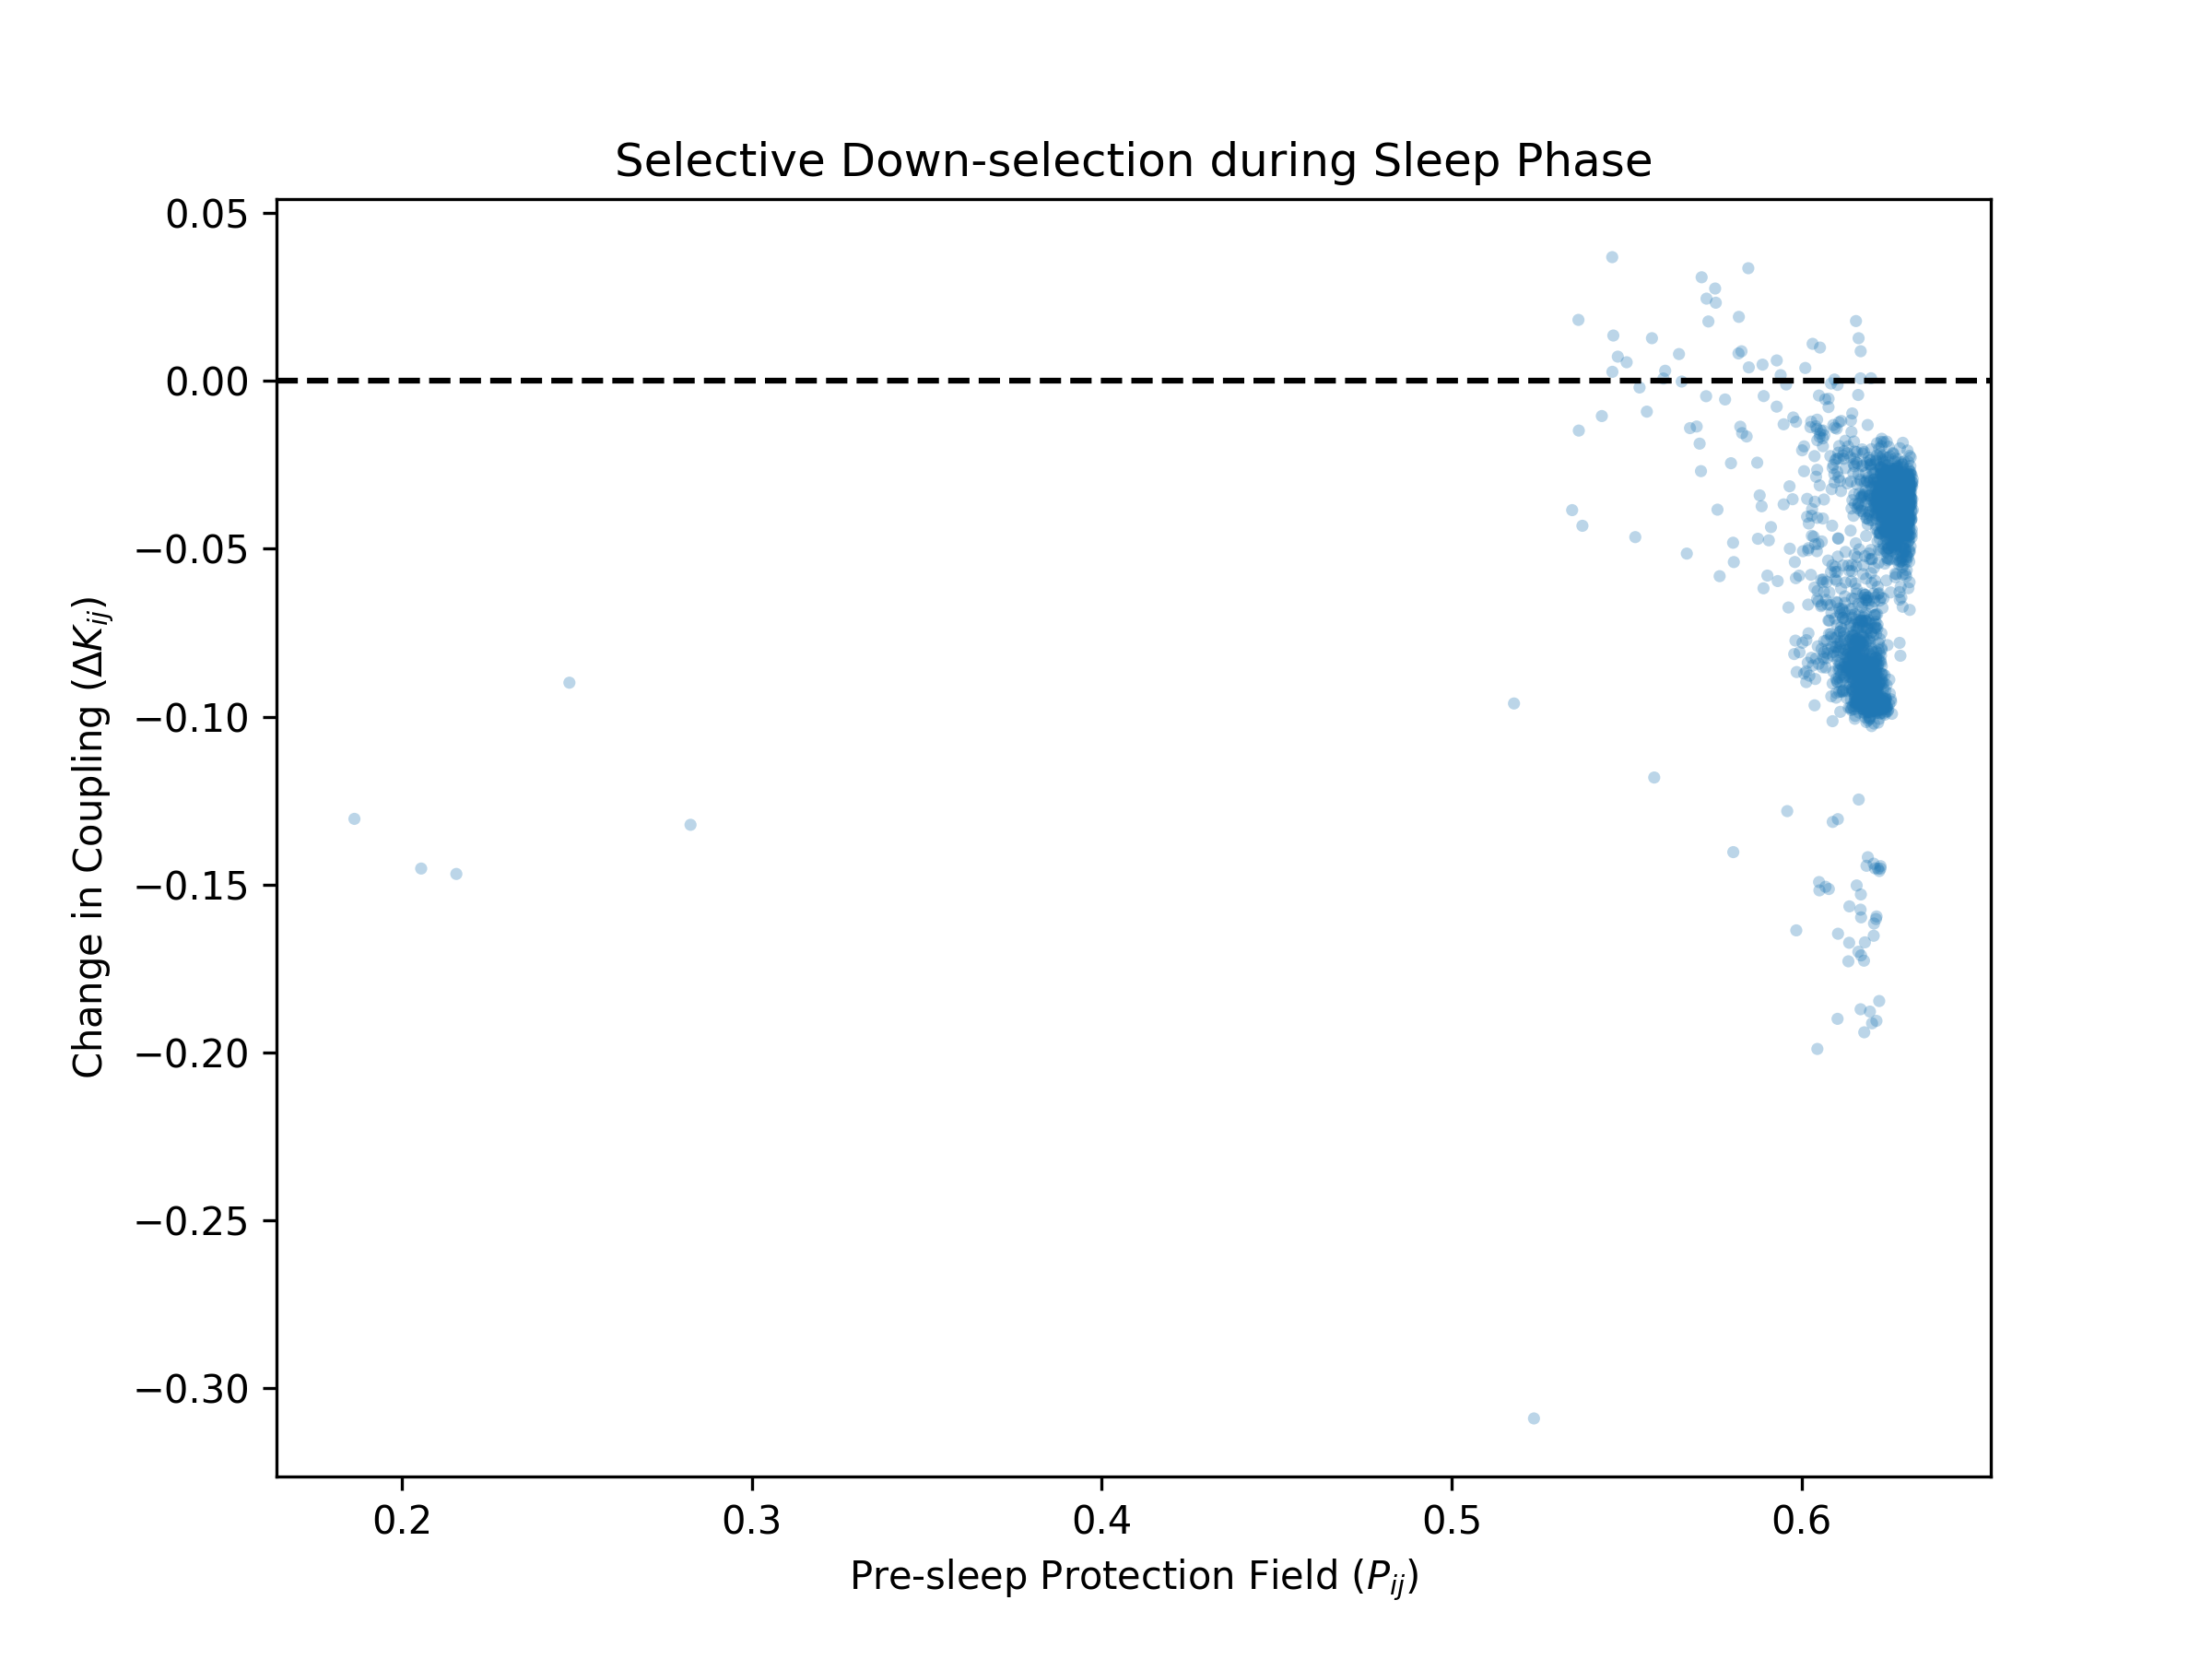
\includegraphics[width=0.72\linewidth]{fig_scatter_selective.png}
\caption{Original selective down-selection diagnostic: coupling change $\Delta K_{ij}$ versus pre-sleep protection field $P_{ij}$. The figure supports only a model-internal selective-protection claim.}
\label{fig:scatter}
\end{figure}

\section{Extended audit sequence}
The v0.2.x audit sequence was designed to test and bound the original mechanism rather than merely add positive examples. Table~\ref{tab:ledger} summarizes the locked phase ledger.

\begin{table}[H]
\centering
\small
\begin{tabular}{p{0.13\linewidth}p{0.30\linewidth}p{0.47\linewidth}}
\toprule
Phase & Role & Locked contribution \\
\midrule
v0.2.0 & Threshold/protection preflight & Threshold-drive candidate identified; sleep-like gate onset and protection controls established. \\
v0.2.1 & Closed-loop hysteresis & Baseline hysteresis-like gap exceeded memoryless control. \\
v0.2.2 & Circadian/multi-cycle audit & Circadian-like permissive gate modulated onset timing; protection remained active. \\
v0.2.3.1 & Perturbation recovery & Acute load pulses evoked gate response; no-gate control suppressed it. \\
v0.2.4 & Topology/noise robustness & Core gate/protection effects persisted across simplified topology and noise settings. \\
v0.2.5 & Conservative envelope & No failure boundary found inside the conservative envelope; claims restricted to that envelope. \\
v0.2.6 & Expanded failure boundary & Failure cases identified; DTTS behavior shown not to be universal. \\
v0.2.7 & Mechanism rescue & Failure modes separated into gate, protection, and unresolved-load boundaries with distinct rescue responses. \\
v0.2.8 & Frozen rescue holdout & Frozen rescue policies generalized for most rescue-sensitive regimes; weak-protection remained unstable. \\
\bottomrule
\end{tabular}
\caption{Claim-bounded DTTS v0.2.0--v0.2.8 audit ledger.}
\label{tab:ledger}
\end{table}

\section{Failure boundaries and frozen rescue holdout}
The v0.2.8 frozen-rescue holdout used six scenario classes, five simplified topologies, and four noise levels, yielding 240 holdout cells. The mean frozen-policy pass rate was 0.7729. Native pass count was 1; rescue holdout pass count was 4; unstable rescue boundary count was 1; persistent failure boundary count was 0. The remaining unstable boundary was weak protection, indicating that structural protection is not merely decorative but a central condition for the modeled selective-renormalization effect.

\begin{figure}[H]
\centering
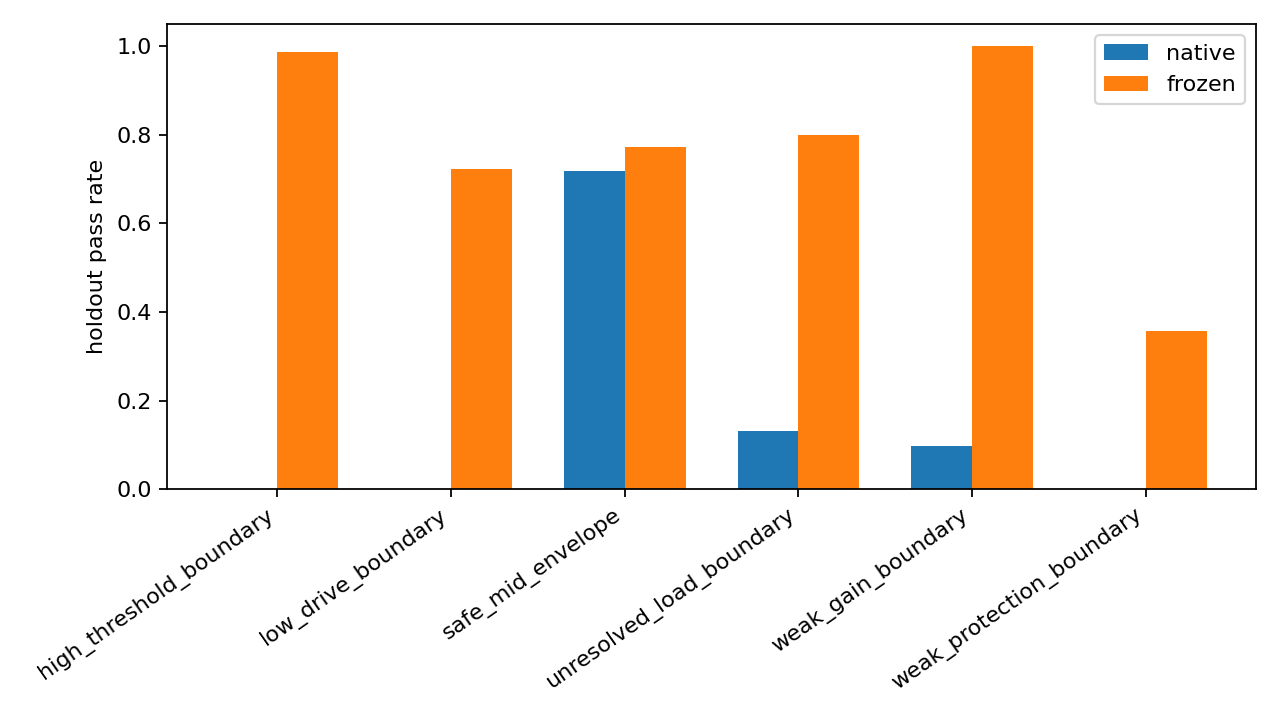
\includegraphics[width=0.93\linewidth]{dtts_v028_frozen_vs_native_pass_rates.png}
\caption{Frozen rescue-policy pass-rate comparison from the v0.2.8 holdout audit. Frozen rescue policies generalized for most rescue-sensitive regimes, while weak-protection remained unstable.}
\label{fig:frozen-pass}
\end{figure}

\begin{figure}[H]
\centering
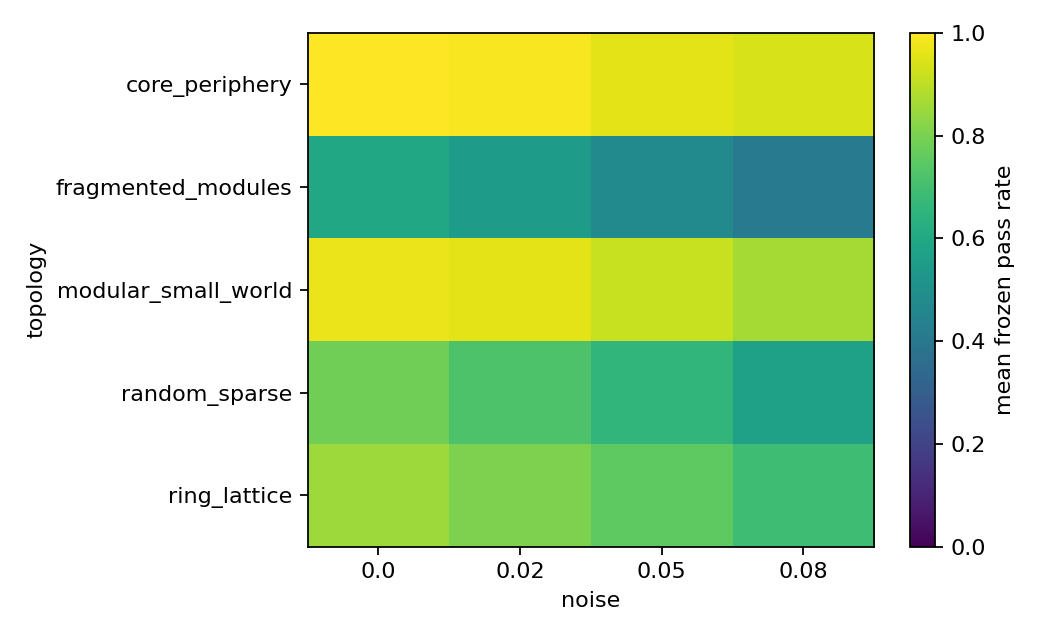
\includegraphics[width=0.82\linewidth]{dtts_v028_topology_noise_holdout_heatmap.png}
\caption{Topology/noise holdout heatmap for frozen rescue-policy generalization. The plot is an internal toy-model robustness diagnostic and should not be interpreted as a biological sleep validation result.}
\label{fig:heatmap}
\end{figure}

\section{Integrated interpretation}
The integrated interpretation is narrower than the original title might suggest but stronger as a research object. DTTS should be read as a network-dynamical recovery-transition prototype with four interacting elements: local load accumulation, thresholded gate onset, structurally aligned selective protection, and regime-dependent rescue sensitivity.

The positive evidence is that the implemented network can show threshold-like gate onset, hysteresis-like persistence, perturbation-recovery response, and selective protection. The negative evidence is equally important: expanded sweeps found conditions under which the desired signatures weaken or fail. Low drive, high threshold, weak gate gain, weak protection, and unresolved-load regimes can disrupt the modeled mechanism. This converts DTTS from a broad sleep claim into a bounded regime-classification framework.

\section{Limitations}
The audits use simplified networks, synthetic load dynamics, synthetic protection fields, and internal toy-model controls. No human data, animal data, polysomnography, EEG, wearable-device data, clinical sleep annotation, pharmacological intervention, or treatment outcome is included. The phrase ``sleep-like'' refers only to a modeled recovery-gate transition, not to physiological sleep.

This manuscript also does not claim that sleep is reducible to a Kuramoto-like network or that biological sleep is generated by the exact variables used here. The model is a hypothesis-generating scaffold for reasoning about recovery-transition motifs in finite adaptive networks.

\section{Data and code availability}
The public GitHub repository is available at \url{https://github.com/yokken0907/dynamical-threshold-theory-of-sleep}. The repository contains manuscript materials, claim-boundary documentation, source-defined Evaluation-Only license files, and evidence packages for the audit sequence. Repository archives should be treated as repository-release artifacts, not as standalone peer-reviewed article identifiers.

\section{Conflict of interest}
The author declares no institutional, financial, or commercial conflict of interest related to this study.

\section*{AI assistance disclosure}
The author used AI assistance for drafting, code generation, numerical-audit scaffolding, and manuscript preparation. The author remains responsible for the final claim boundary, interpretation, and release decisions.

\section{Conclusion}
DTTS v0.3.1 integrates the original model manuscript and the later audit sequence. The resulting claim is intentionally bounded: in the implemented finite adaptive-network toy model, sleep-like recovery-transition motifs can arise through local load accumulation, thresholded gate onset, and structurally aligned selective protection, while extended audits identify both rescue-sensitive regimes and failure boundaries. This is a claim-bounded network-dynamical prototype, not a biological or clinical theory of sleep.

\begin{thebibliography}{99}
\bibitem{Tononi2003} Tononi, G., and Cirelli, C. (2003). Sleep and synaptic homeostasis: a hypothesis. \textit{Brain Research Bulletin}, 62(2), 143--150.
\bibitem{Tononi2006} Tononi, G., and Cirelli, C. (2006). Sleep function and synaptic homeostasis. \textit{Sleep Medicine Reviews}, 10(1), 49--62.
\bibitem{Cirelli2015} Cirelli, C., and Tononi, G. (2015). Sleep and Synaptic Homeostasis. \textit{Sleep}, 38(10), 1615--1624.
\bibitem{Tononi2014} Tononi, G., and Cirelli, C. (2014). Sleep and the Price of Plasticity. \textit{Neuron}, 81(1), 12--34.
\bibitem{Vyazovskiy2011} Vyazovskiy, V. V., et al. (2011). Local sleep in awake rats. \textit{Nature}, 472(7344), 443--447.
\bibitem{Krueger2019} Krueger, J. M., et al. (2019). Local Sleep. \textit{Sleep Medicine Reviews}, 43, 14--21.
\bibitem{Siclari2018} Siclari, F., et al. (2018). Local aspects of sleep and wakefulness. \textit{Current Opinion in Neurobiology}, 44, 222--227.
\bibitem{Borbely2022} Borbely, A. A., et al. (2022). The two-process model of sleep regulation. \textit{Journal of Sleep Research}, 31(6), e13598.
\bibitem{Deboer2018} Deboer, T. (2018). Sleep homeostasis and the circadian clock. \textit{Neurobiology of Sleep and Circadian Rhythms}, 5, 68--77.
\bibitem{Acebron2005} Acebron, J. A., et al. (2005). The Kuramoto model. \textit{Reviews of Modern Physics}, 77(1), 137--185.
\bibitem{Hong2002} Hong, H., et al. (2002). Synchronization on small-world networks. \textit{Physical Review E}, 65(2), 026139.
\end{thebibliography}

\end{document}
